\begin{quotation}
	``I don’t need a hard disk in my computer if I can get to the server faster… carrying around these non-connected computers is byzantine by comparison.'' - \parencite{jobs.1997}
\end{quotation}

Die IT-Industrie hat sich im letzten Jahrzehnt massiv verändert. Durch neue Technologie ist es immer leichter möglich, Dienste und Lösungen zentral zusammenzulegen. Wo früher noch dedizierte Server für spezielle Anwendungen genutzt wurden, versucht man heute Szenarien dieser Art zu vermeiden.

Durch immer leistungsstärkere Hardware ist ein einzelner Server in der Lage, eine Vielzahl von Aufgaben parallel zu bearbeiten. Im ersten Schritt führte dies zu der Virtualisierung der Servern selber, mit modernen Cloud-Lösungen geht man sogar noch einige Schritte weiter. Die komplette Infrastruktur und Plattform wird vor dem Nutzer verborgen, es besteht nur noch Kontrolle über die spezifische Software. Wo diese läuft oder welche Leistung notwendig ist, wird dynamisch vom Cloud System bestimmt.

Ebenfalls entstehen neue Anforderung durch den erstarkenden Markt von mobilen Geräten. Anwendungen müssen von tausenden Smartphones oder Tablets gleichzeitig angesprochen werden können und diverse Betriebssysteme unterstützten. 

Software-Anbieter sind nicht mehr in der Lage vorhersagen zu können, ob der Nutzer einen Desktop PC mit umfassender Leistung oder ein veraltetes Handy mit nur minimalen Systemfunktionen zur Verfügung hat. Informationen über Hauptspeicher, Festplatten, CPU oder Grafikeinheiten sind meistens Unbekannte, die nicht vorausgesetzt werden können. Aus diesem Grund werden rechenintensive Aufgaben auf der Serverseite erledigt, was zusätzlich zu enormen Anforderungen an die Server führt.

Dedizierte Server kommen hierbei schnell an ihre Grenze. Wird der Dienst häufig genug verwendet, kommt selbst die leistungsstärkste Maschine irgendwann an ihre Grenzen. Außerdem würde diese ungeheure Ressourcen verbrauchen, die aber nur selten komplett ausgelastet würden. 
Zentralisierte Rechenzentren würden bereits viele dieser Probleme lösen, kommen aber bei internationalen Anwendungen ebenfalls schnell an ihre Grenzen. Nur auf ein Land beschränkte Services stellen kein Problem dar, aber sobald eine Software international genutzt werden soll, müssen Rechenzentren auf jedem Kontinent zur Verfügung stehen. Alternative müssten hohe Latenzzeiten hingenommen werden, die aber heutzutage vollkommen unakzeptabel sind.

Neben diesen funktionalen Problemen sind nur wenige Firmen bereit, die Ausrüstung und das Personal für einen eigenen Serverpark aufzubringen.

Die Cloud bietet hierbei eine angenehme Lösung, diese klassischen Probleme dem Kunden abzunehmen.

\begin{figure}[hbt]
	\centering
	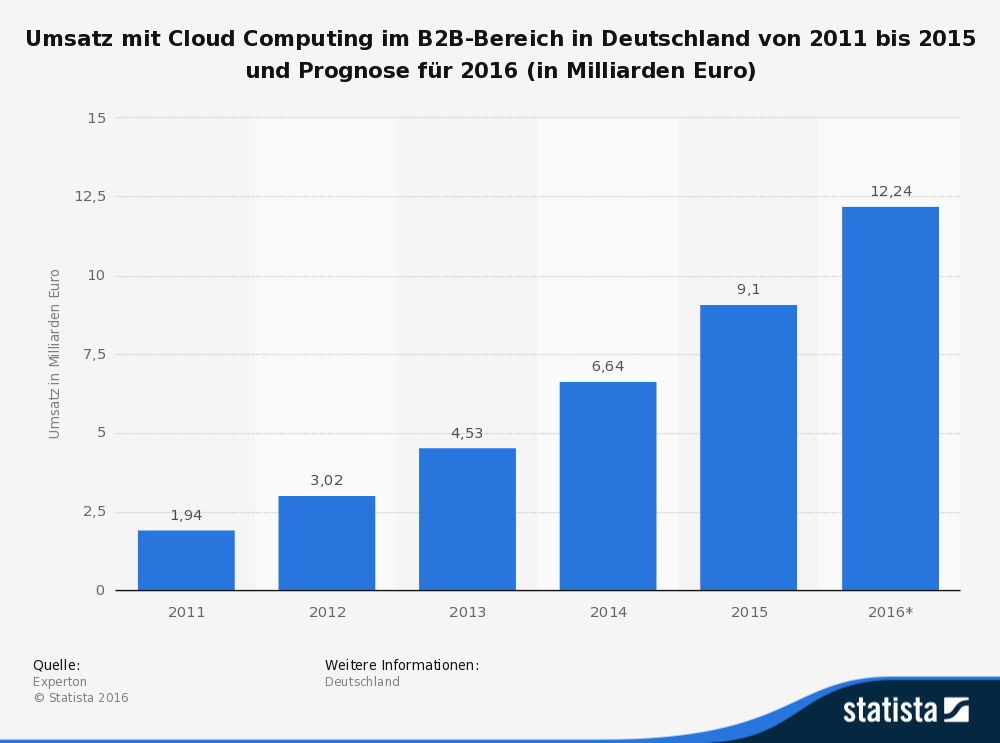
\includegraphics[scale=0.5]{images/cloud-computing-market}
	\caption{Umsatz mit Cloud Computing im B2B-Bereich in Deutschland von 2011 bis 2015 und Prognose für 2016 \parencite{statistia.2015}}
	\label{fig:cloudmarket}
\end{figure}

Wie man \autoref{fig:cloudmarket} entnehmen kann, passen sich die verschiedenen Vendoren an die neuen Herausforderungen an und fokussieren immer mehr auf den Cloud-Computing-Markt.

Leider entstehen hierdurch wieder neue Probleme: Die Kontrolle über nutzerspezifische Daten geht verloren. Durch das Deployment der Anwendung auf verschiedene Server und die Verteilung der Daten auf verschiedene Datenbanken ist es für den Nutzer schwierig geworden, den Datenweg nachzuvollziehen.

Dies wird besonders zum Problem, wenn rechtlich geschützte Daten in der Cloud verwendet werden sollen. Ebenfalls gibt es sensitive Geschäftsdaten, die Firmen nur ungern aus der Hand geben möchten und die nicht ins unsichere Internet gelangen dürfen.
Zum Teil kann dies durch bessere Sicherheitslösungen und Verschlüsselung behoben werden, aber oft müssen zumindest die Datenbanken beim Kunden vor Ort bleiben. 

Um auch diesen Anforderungen gerecht zu werden, entstehen immer häufiger so genannte Hybrid Cloud Modelle. Bei diesen findet ein Teil der Geschäftsprozesse in der öffentlichen Cloud statt und sicherheitskritische Softwareteile werden lokal vom Nutzer selbst gehostet. Ebenfalls besteht bei diesen Lösungen die Möglichkeit, dass Performance Spitzen in der Cloud bearbeitet werden, sodass spontan zusätzliche Leistung alloziert werden kann.

Im Kontext dieser Arbeit soll untersucht werden, inwiefern eine Cluster Speicherlösungen an eine Public Cloud angebunden werden kann, sodass selten verwendete Daten automatisch in die Cloud ausgelagert werden und Anwendungen auf den nicht öffentlichen Speicher zugreifen können.  